\documentclass[11pt,a4paper,openany]{book}

\makeatletter\def\input@path{{../_shared/}}\makeatother
\usepackage{course}

\begin{document}
\raggedbottom

\coursetitle{Compsys}{BA4}{2025--2026}

\tableofcontents
\clearpage


% ===========================================================
\chapter{Lecture 11 --- File Systems}
% ===========================================================

\section{Motivation : Persistance}

\begin{defnbox}[title={Persistance}]
État qui \textbf{survit au processus qui l'a créé}~: terminaison du processus, redémarrage, coupure de courant. Sans cela, tout réside en DRAM (volatile) et disparaît à l'extinction.
\end{defnbox}

Un file system donne aux utilisateurs quatre capacités clés sur le stockage persistant~:
\textbf{Nommer} — \textbf{Organiser} — \textbf{Partager} — \textbf{Protéger}.

\section{Abstractions}

\begin{defnbox}[title={Inode}]
Structure on-disk représentant un fichier ou dossier~: \textbf{métadonnées} (taille, propriétaire, permissions, timestamps) + \textbf{pointeurs de blocs} vers les données.
\end{defnbox}

\begin{defnbox}[title={Répertoire}]
Fichier spécial dont le contenu est un tableau de paires \texttt{(nom, numéro d'inode)}. Un flag dans l'inode restreint l'API (pas de \texttt{write()} direct). Toute l'arborescence repose sur \emph{une seule} abstraction~: le fichier.
\end{defnbox}

\begin{keybox}
\textbf{Résolution de chemin} \texttt{/tmp/test.txt}~: inode racine $\to$ data racine $\to$ inode \texttt{tmp} $\to$ data \texttt{tmp} $\to$ inode \texttt{test.txt} $\to$ blocs de données. \textbf{5 lectures disque minimum.}
\end{keybox}

\begin{figure}[h]
  \centering
  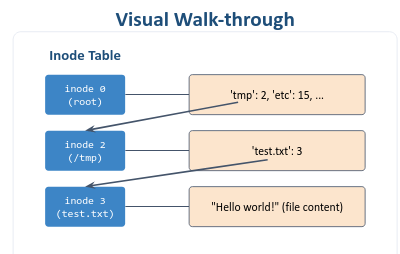
\includegraphics[width=0.6\textwidth]{images/accessing-path-using-inodes.png}
  \caption{Walk de chemin via la table d'inodes.}
\end{figure}

\section{File Descriptors}

\begin{warnbox}
Refaire le walk à chaque \texttt{read()} coûte $250{,}000 \times 5 = \mathbf{1{,}25\,\text{M}}$ lectures disque pour un fichier de 1\,Go lu en blocs de 4\,Ko.
\end{warnbox}

\begin{defnbox}[title={File Descriptor (fd)}]
Entier par-processus. À l'\texttt{open()}, l'OS fait le walk \emph{une seule fois}, met l'inode en cache, et renvoie un fd. Les \texttt{read()}/\texttt{write()} suivants utilisent directement ce cache. fd~0/1/2 = STDIN/STDOUT/STDERR.
\end{defnbox}

\begin{figure}[h]
  \centering
  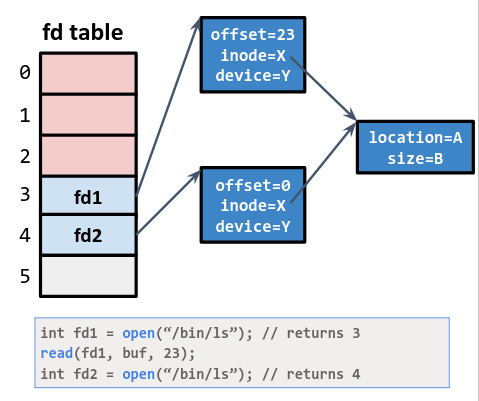
\includegraphics[width=0.55\textwidth]{images/fd-table.png}
  \caption{Table de fd par processus. fd1 et fd2 partagent le même inode mais ont des offsets indépendants.}
\end{figure}

\section{Layout Disque}

\begin{figure}[h]
  \centering
  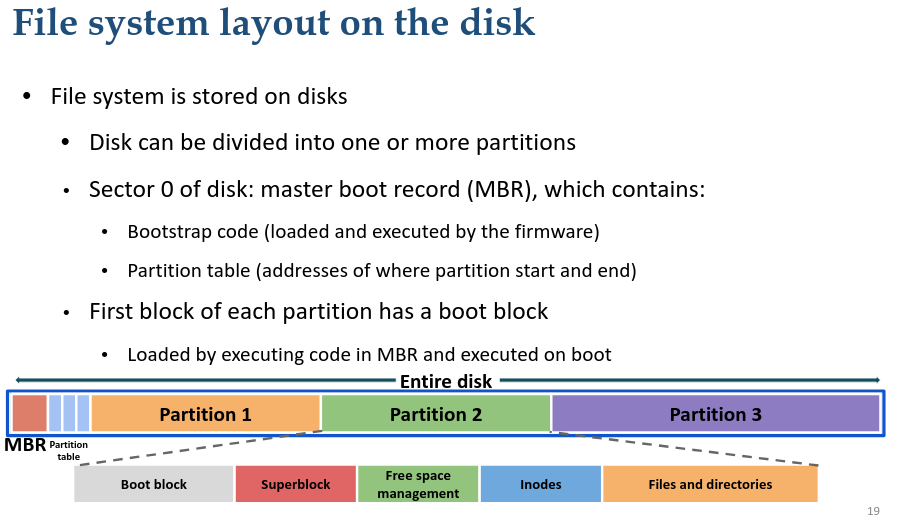
\includegraphics[width=0.88\textwidth]{images/partition-structure.png}
  \caption{MBR (secteur 0) $\to$ table de partitions $\to$ chaque partition~: \textbf{boot block | superblock | bitmap espace libre | table d'inodes | blocs de données}.}
\end{figure}

\begin{defnbox}[title={Superblock}]
Métadonnées de la partition~: nombre d'inodes/blocs, emplacement de la table d'inodes, bitmaps libres. Lu en premier au montage~; sa corruption rend la partition illisible.
\end{defnbox}

\texttt{mount <device> <dir>} rattache la racine d'un système de fichiers à un point de montage existant. Tout répertoire peut être un point de montage.

\section{Allocation de Blocs}

\begin{center}
\begin{tabular}{lll}
\toprule
\textbf{Méthode} & \textbf{Avantage} & \textbf{Inconvénient} \\
\midrule
Contiguous  & Lecture séquentielle rapide & Fragmentation, extension coûteuse \\
Linked list & Extension/suppression facile & Accès aléatoire O(n) \\
FAT         & Liens hors des blocs        & Table entière en mémoire \\
\textbf{Multi-level} & O(1) petits fichiers, $\le$4 I/O grands & Léger overhead très grands fichiers \\
\bottomrule
\end{tabular}
\end{center}

\begin{defnbox}[title={Multi-Level Indexing (Unix)}]
L'inode contient~: 12 pointeurs \textbf{directs} + 1 \textbf{simple-indirect} + 1 \textbf{double-indirect} + 1 \textbf{triple-indirect}. Avec blocs de 4\,Ko et pointeurs de 4 octets (1024 ptr/bloc)~:
\[
  12 \times 4\,\text{Ko} = 48\,\text{Ko}
  \quad 1024 \times 4\,\text{Ko} = 4\,\text{Mo}
  \quad 1024^2 \times 4\,\text{Ko} = 4\,\text{Go}
  \quad 1024^3 \times 4\,\text{Ko} = 4\,\text{To}
\]
\end{defnbox}

\begin{figure}[h]
  \centering
  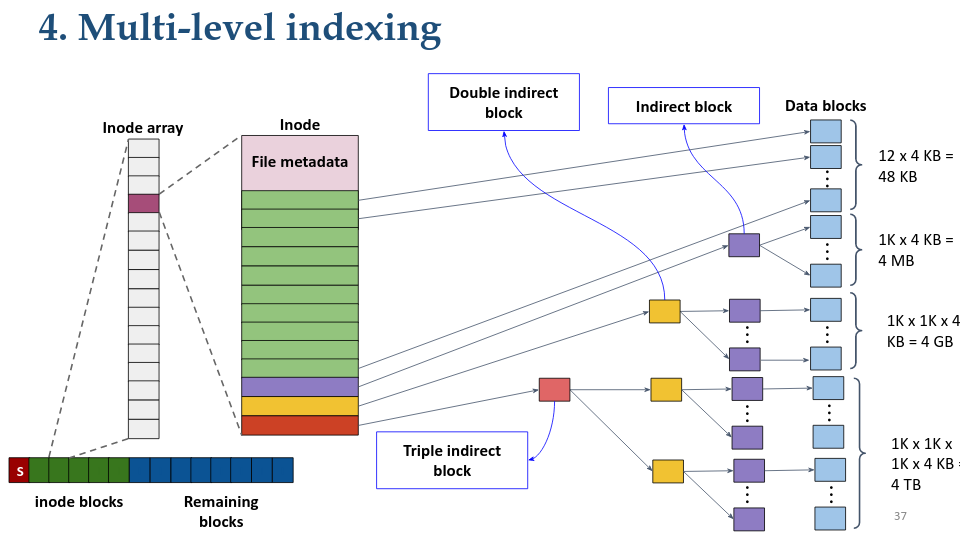
\includegraphics[width=0.88\textwidth]{images/multi-level-indexing.png}
  \caption{Structure multi-niveau. Les petits fichiers n'utilisent que les pointeurs directs~; les grands fichiers traversent jusqu'à 3 niveaux d'indirection (4 lectures disque max).}
\end{figure}

\begin{figure}[h]
  \centering
  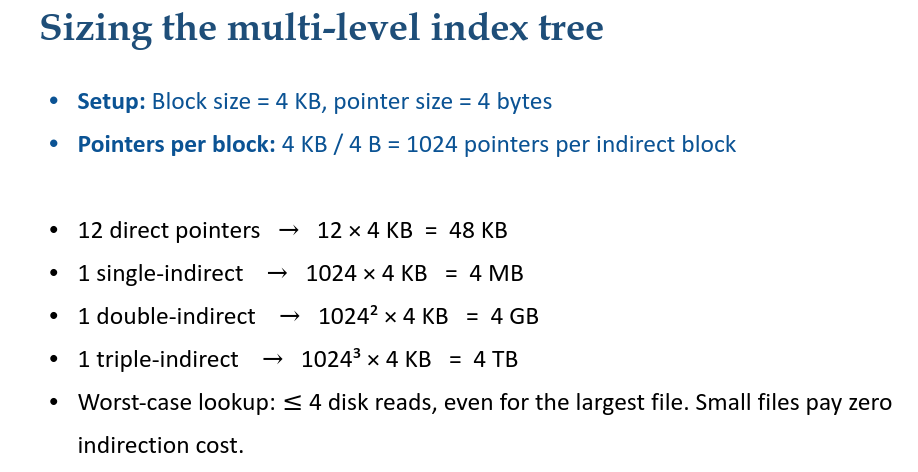
\includegraphics[width=0.72\textwidth]{images/sizing-muti-level-index-tree.png}
  \caption{Calcul des tailles maximales (blocs 4\,Ko, pointeurs 4 octets~: 1024 ptr/bloc).}
\end{figure}

\section{Coût des Opérations Fichier}

\begin{keybox}[title={Nombre d'opérations disque}]
\begin{itemize}
  \item \textbf{open()} (chemin à 2 niveaux)~: 5 lectures.
  \item \textbf{read()} (n\textsuperscript{ème} bloc)~: 1 lecture (data) + 1 écriture (inode atime). Premier appel~: +1 lecture inode.
  \item \textbf{write()} (nouveau bloc)~: 2 lectures + 3 écritures (bitmap×2, inode, data).
  \item \textbf{create()}~: +{\raise.17ex\hbox{$\scriptstyle\sim$}}6 ops supplémentaires (bitmap inode, nouvel inode, data dir, inode dir).
\end{itemize}
\end{keybox}

\begin{keybox}[title={Block Cache}]
Le cache disque (DRAM) élimine la majorité des I/O. Taux de hit $>99\%$ fréquents $\Rightarrow$ jusqu'à \textbf{1000×} de gain. C'est pour cela qu'éviter les I/O est la priorité numéro 1.
\end{keybox}

\clearpage
\section*{Résumé}
\addcontentsline{toc}{section}{Résumé}

\begin{keybox}
\begin{itemize}
  \item \textbf{Persistance}~: état qui survit au processus. DRAM volatile $\neq$ disque non-volatile.
  \item \textbf{4 buts FS}~: Nommer, Organiser, Partager, Protéger.
  \item \textbf{Inode}~: métadonnées + pointeurs de blocs. Un inode par fichier/dossier.
  \item \textbf{Répertoire}~: fichier dont le contenu est un tableau \texttt{(nom, inode)}.
  \item \textbf{fd}~: entier par-processus cachant \texttt{(inode, offset)} après \texttt{open()}. fd 0/1/2 = STDIN/STDOUT/STDERR.
  \item \textbf{Path walk}~: 5 lectures pour \texttt{/tmp/test.txt} — coûteux si répété à chaque \texttt{read()}.
  \item \textbf{Layout partition}~: boot | superblock | bitmap | inodes | data.
  \item \textbf{Multi-level indexing}~: 12 directs (48\,Ko) + single (4\,Mo) + double (4\,Go) + triple (4\,To). $\le$4 lectures extra au pire.
  \item \textbf{Block cache}~: hit rate $>99\%$ $\Rightarrow$ 1000× speedup. Éviter les I/O est critique.
\end{itemize}
\end{keybox}


\end{document}
